\chapter{Clases}
\section{Modelado de clases}
Nuestra primer idea al modelar la soluci�n, fue identificar los diversos componentes logicos presentes en el sistema. De esta manera pudimos identificar la existencia de grupos de funcionalidades que se pod�an agrupar. Consideramos la existencia de los siguientes componentes:

\begin{figure}[H]
\centering
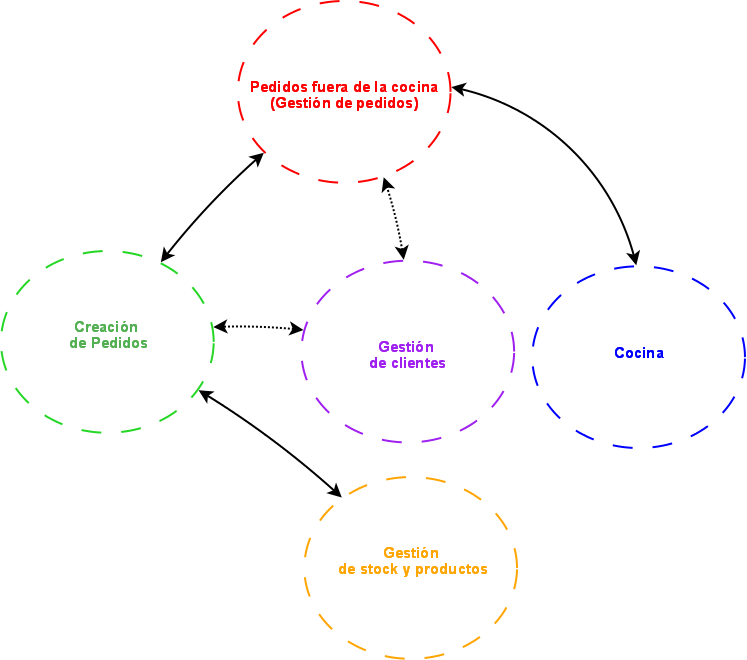
\includegraphics[height=10cm]{./figuras/divisionModelo.png}
\caption{Esquema de componentes l�gicos}
\end{figure}

\begin{itemize}
\item Pedidos fuera de la cocina: Este componente agrupa las funcionalidades del ingreso, despacho, consulta de estado y otros aspectos que involucren a las partes del ciclo de vida que no ocurran en el ambito de la cocina.
\item Creaci�n de pedidos: Aqu� se agrupan aquellas funcionalidades que hacen posible que se creen e ingresen al sistema nuevos pedidos. Podr�a considerarse parte de Pedidos fuera de la cocina, pero sin embargo la creaci�n tiene una logica bastante compleja de estimaci�n de tiempos, chequeo de stock, entre otras cosas que nos llevaron a considerarlo como un componente separado.
\item Gesti�n de clientes: Este componente permite realizar las validaciones de clientes asi como tambi�n las altas, bajas y modificaciones de clientes
\item Cocina: Aqui se engloban las funciones que permiten guiar la preparaci�n y cocci�n de un pedido.
\item Gesti�n de stock y productos: En este componente se engloba el ABM de stock y el ABM de productos
\end{itemize}

Esta divisi�n sirve para gu�a pero no es estrictamente asi, ya que por ejemplo la cancelaci�n es un evento que toca tanto a la cocina como a los pedidos fuera de esta, por otro lado el Pedido como tipo de datos es utilizado por todos los componentes en mayor o menor medida. No obstante creemos que esta divisi�n en componentes sirve para mostrar el enfoque que se le dio al dise�o

\section{Pedidos fuera de la cocina}
Como dijimos este componente tiene por responsabilidad el manejo de la vida de los pedidos que estan fuera de la cocina (por cocina entendemos no solo al horno, sino tambi�n a la preparaci�n de los pedidos).

Nuestra idea fue tener un coordinadorDePedidos que siga el patron Fa�ade, de modo que muestre a la interfaz grafica una intrefaz \textit{``gruesa''} con las funciones que se realizan dentro del componente. Esta clase no va a tener gran inteligencia, sino que se limitara a propagar la llamada originada por la interfaz grafica a la clase responsable de manejar esa llamada. As�, por ejemplo para ver el estado de un pedido o ingrear un nuevo pedido se deber� pasar por esta clase.
La idea de esta clase es desacoplar la interfaz grafica de las clases que manejan a los pedidos fuera de la cocina. Si bien esta clase para tener baja cohesi�n, al mirarla de cerca vemos que lo �nico que hace es derivar las llamadas. De este modo si bien a trazo grueso parece tener una interfaz con poca cohesi�n, esta nos permite lograr un menor grado de acoplamiento entre la interfaz y el sistema en si. Por esta raz�n decidimos pese al aparente conflicto con la cohesi�n, decidimos mantener esta clase.
Ademas el coordinadorDePedidos se comunica con el componente encargado de crearPedidos, haciendo de puente entre ambos componentes.

Cuando se realiza un pedido de ingreso, el coordinador se encarga de pedir que se genere el pedido, y en caso de que se pueda crear, lo deriva al controladorDePreIngreso, cuya funci�n es determinar si el pedido debe ir a la cola de listos, porque no hay nada que preparar, ni cocinar, o lo tiene que mandar al controlador de ingreso, porque hay algo que cocinar o preparar. Este comportamiento se hizo con la intenci�n de permitir en un futuro incorporar otros productos ademas de pizzas o empanadas. Por ejemplo, podrian venderse ensaladas, las cuales no requieren de cocci�n, pero si de preparaci�n. Por eso decidimos que un producto tuviera atributos de cocinable y preparable.

El controladorDeIngreso se encarga de mantener la cola de ingreso, asi como de suministrar los pedidos al CoordinadorDeCocina, para que este los distribuya al preparador o al coordinador de horno.
El coordinadorDeIngreso puede recibir recibir una solicitud de un pedido de cierto tipo por parte del CoordinadorDeCocina, por ejemplo puede recibir una solicitud del proximo pedido que contenga algun producto del tipo empanada.
Por otro lado, cada vez que ingresa un nuevo pedido, el controladorDeIngreso pregunta al CoordinadorDeCocina si puede recibir dicho pedido. Esta funcionalidad sirve para aquellos casos en los que por ejemplo no hay ningun pedido ingresado con empanadas y el maestro empanadero esta ocioso. Si llega un nuevo pedido con empanadas, el maestro debe ser notificado, por esta razon el ControladorDeIngreso pregunta si debe encolar el pedido o hay alguien que lo vaya a preparar.

Otra clase de este componente, es el ControladorDeListos, este controlador va a recibir los pedido listos y va a encargarse en el momento del despacho de decidir que hacer con el pedido. Por ejemplo si es un pedido con delivery hay que marcar que salio con el delivery, y si era local hay que marcarlo como finalizado.

La clase controladorDeEntragas contiene a todos los pedidos cuya entrega esta pendiente, y se encargan de finalizar el pedido cuando se notifica la entrega.

Por ultimo el controladorPedidosMesa monitorea los pedidos entregados a una cierta mesa, permitiendo que al cerrar la mesa se fijen sus formas de pago.

La clase controladorDeIngreso es abstracta porque consideramos que la estrategia con la que se maneja la cola de ingreso podria cambiar, de esta manera la versi�n propuesta por nosotros en la etapa de especificaci�n es implementada por controladorDeIngresoStandard. Utilzar una clase abstracta nos permite lograr flexibilidad si se quiere cambiar de politica de manejo de esta cola, por ejemplo usando un manejo del tipo mas corto primero.

El resto de las clases no son abstractas, esto si bien parece no cumplir con el principio \textit{DIP}, al mirar mas de cerca notamos que son clases bastante tontas, solo almacenan cierto tipo de pedidos y luego hacen sets de algunos atributos de algun pedido que contienen, por lo que es de esperarse que su comportamiento no se modifique, y dado lo poco que hace cada una de ellas, en el caso de tener que modificar, no deber�an generar un impacto significativo al modelo.

\textcolor{Red}{TODO: interacciones de estas clases con la GUI}

\textcolor{Red}{TODO: explicacion de metodos importantes}
\subsection{Modelado de escenarios}
\textcolor{Red}{TODO: escenarios que muestren el comportamiento de estas clases en los fenomenos pedidos en el enunciado}

\textcolor{Red}{TODO: pseudocodigos que muestren algoritmos como por ej la busqueda de un pedido para ingresar}

\section{Creaci�n y registro de pedidos}
En este componente se agrupan las clases que entran en juego al momento de crear un nuevo pedido.

La clase GeneradorDePedidos sirve de punto de entrada a este componente. El mismo posee el m�todo generarPedido, que es invocado por el Coordinador de pedidos, a fin de que se ingrese al sistema un nuevo pedido.

El Generador se encarga de llamar al controladorDeStock para que verifique que el stock existente sea capaz de satisfacer al pedido. Ademas el generador realiza el decremento del stock, y se encarga de realizar el callback a la gui en caso de que un insumo quede por debajo de su stock critico. %TODO: callback como?

Luego de que se regisr� el decremento de stock, el Generador se encarga de llamar al EstimadorDeTiempos. Esta clase es abstracta, ya que pensamos que como la pizzeria desea ir refinando estas estimaciones, es probable que la forma de estimar se modifique de forma periodica. Por lo tanto, decidimos aplicar el \textit{Strategy pattern} a fin de poder lograr varias estrategias de estimaci�n. La Estimaci�n desarrollada en \ref{modifEstim} es implementada por la clase EstimadorBasico.

\textcolor{Red}{TODO: interacciones de estas clases con la GUI}

\textcolor{Red}{TODO: explicacion de metodos importantes}
\subsection{Modelado de escenarios}
\textcolor{Red}{TODO: escenarios que muestren el comportamiento de estas clases en los fenomenos pedidos en el enunciado}

\textcolor{Red}{TODO: pseudocodigos que muestren algoritmos como por ej estimacion de tiempos}



\section{Diagrama de clases}
\begin{landscape}
\begin{figure}
\centering
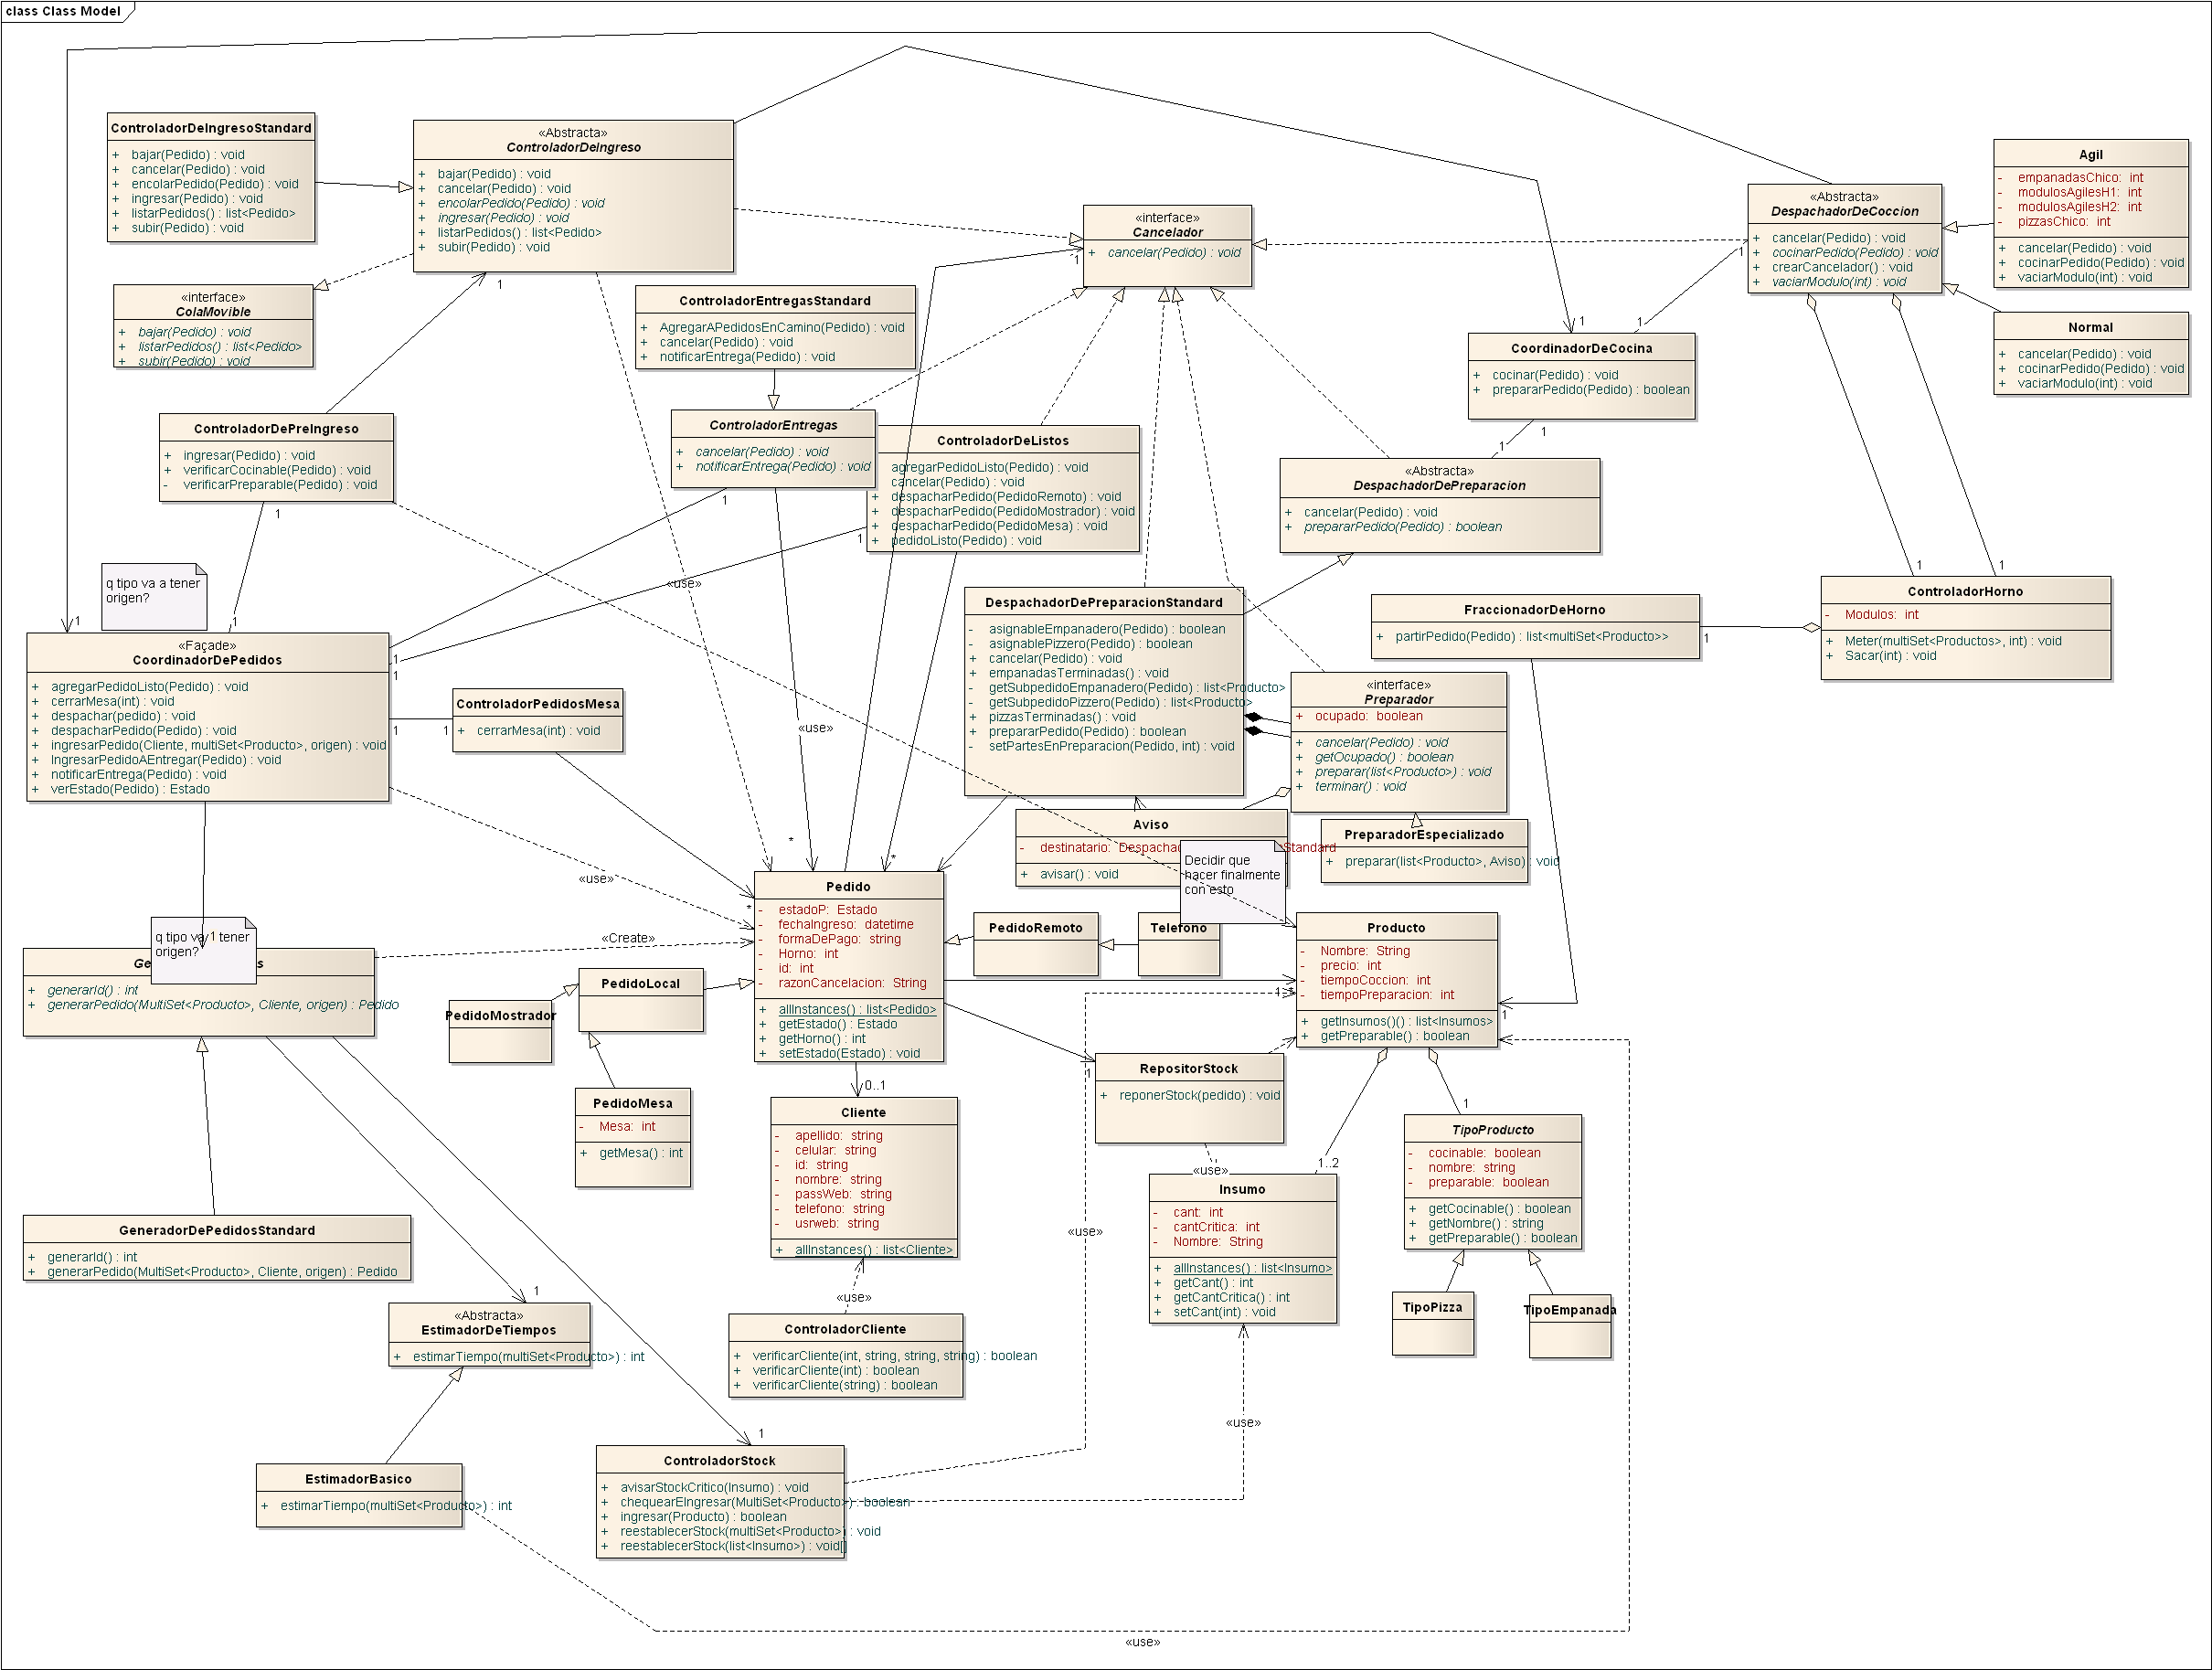
\includegraphics[height=18cm]{./figuras/clases.png}
\end{figure}
\end{landscape}

\section{Explicaci�n de las clases}
\clase
{ABMproductos}
{Esta clase se encarga de realizar las altas, bajas y modificaciones de los productos}
{}{}

\clase
{ABMstock}
{Esta clase se encarga de realizar las altas, bajas y modificaciones de los insumos}
{}{}

\clase
{Agil}
{Especializaci�n de gestor de horno, permite aplicar la politica agil}
{}{}

\clase
{Aviso}
{Clase utilizada para realizar el \textit{callback} desde el gestor de horno hacia el despachador de preparaci�n, es la encargada de ejecutar el metodo del despachador que lo notifica de que se termino de preparar algo. Esta clase permite que el despachador no necesite saber quien le avisa, y por lo tanto permite que los preparadores no requieran de metodos diferenciados para avisar que se terminaron de preparar las pizzas, o las empanadas}
{}{}

\clase{Cliente}
{Esta clase representa a un cliente, conteniendo todos los datos del mismo.}
{}{}

\clase{ColaListos} %FIXME: nombre poco feliz
{Esta clase contiene a los pedidos que ya estan listos. Su responsabilidad es la de conocer a todos los que estan en este estado, a fin de que despachar un pedido se haga desde esta clase}
{}{}

\clase
{ControladorDeIngreso}
{Controla la cola de ingreso, la cual puede ser modificada por el encargado de pedidos. Cuando algun preparador queda libre, envia el proximo pedido a preparar}
{}{}

\clase
{ControladorCliente}
{El controlador de cliente tiene por responsabilidad encargarse de autentificar un usuario}
{}{}

\clase
{ControladorStock}
{El controlador de stock, tiene por responsabilidad chequear la disponibilidad de insumos al momento de un ingreso, asi como la de hacer el decremento del stock al ingresar un pedido, generando el aviso de stock critico en caso de ser necesario.}
{}{}

\clase
{CoordinadorDePedidos}
{El coordinador de pedidos se encarga de controlar el ingreso de pedidos, y su ciclo de vida fuera de la cocina}
{}{}

\clase
{DespachadorDePreparaci�n}
{Esta clase tiene por responsabilidad manejar la cola de pedidos que se estan preparando, recordemos que puede existir una cola de preparaci'on si hay pedidos mixtos a la espera de uno de los maestros. El controlador de ingresos distribuye los pedidos a los distintos preparadores y despacha cada pedido a su gestor de horno correspondiente cuando ya esta preparado.}
{}{}

\clase
{EstimadorDeTiempos}
{El estimador de tiempos, como lo dice su nombre, se encarga de estimar el tiempo de preparacion y cocci�n de un pedido}
{}{}

\clase
{GeneradorDePedidos}
{Esta clase se encarga de crear pedidos, creando pedidos de solo bebidas o con comida segun los productos}%FIXME: justificacion
{}{}

\clase
{GestorHorno}
{Clase abstracta que permite implementar diferentes politicas para el manejo del horno}
{}{}

\clase
{Insumo}
{Contiene la informaci�n de los distintos insumos de la pizzer�a}
{}{}

\clase
{Normal}
{Permite implementar la politica normal de manejo del horno}
{}{}

\clase
{Pedido}
{Contiene la informaci�n de cada pedido}
{}{}

